\documentclass[12]{article}
\usepackage[utf8]{inputenc}
\usepackage{float}
\usepackage{hyperref}
\usepackage{graphicx}
\date{\today}
\author{Carlos Bergillos, Roger Vilaseca, Adrià Cabeza}
\title{Creación de dietas para ancianos: \\ Sistemas Basados en el conocimiento \\
	\large IA FIB @ UPC}
\usepackage[margin=1.25in]{geometry}
\usepackage{listings}
\lstset{
	    basicstyle=\ttfamily,
	    showstringspaces=false,
	    commentstyle=\color{orange},
	    keywordstyle=\color{blue},
	    breaklines=true,numbers=none,
	    stringstyle=\color{red}, tabsize=3,   
	    showstringspaces=false,
	    columns=flexible,
	}
\begin{document}
\maketitle
%\vspace*{\fill}
%\begin{center}
%
\includegraphics[scale=0.5]{images/UPClogo.png}
%\end{center
\newpage
\tableofcontents
\newpage
\section{Introducción}
Los \textbf{sistemas basados en el conocimiento (SBC)} son la parte de la Inteligencia Artificial donde se intenta hallar una solución utilizando el conocimiento. Hay ciertos problemas en la vida real que no se pueden resolver sin tener conocimiento específico sobre los elementos del dominio. 
\par
El motivo de esta práctica es comprender estos modelos de IA así que hemos atacado un problema con esta técnica: creación de menús para ancianos dependiendo de sus necesidades nutricionales y requisitos médicos. 
\par
Hemos desarrollado una ontología capaz de almacenar la información sobre los platos, los ingredientes, los nutrientes, las enfermedades y las limitaciones con \textbf{Protégé} y un sistema de reglas que describen el proceso de toma de decisiones usando \textbf{CLIPS}.
\par
Para atacar el problema de una manera adecuada hemos utilizado las diferentes fases de la metodología de ingeniería del conocimiento: 

\begin{itemize}
\item Identificación, donde identificaremos el problema y sus características y requisitos. Además también concretaremos el dominio para poder identificar las fuentes de conocimiento necesarias para su desarrollo.
\item Conceptualización, donde describiremos en profundidad los conceptos que intervienen en el dominio del problema y la descomposición de este último en subproblemas. 
\item Formalización, donde partiendo de los conceptos de la fase anterior, procediremos a su formalización desarrollando una ontología. También, para la resolución del problema formalizaremos el conocimiento y una metodología de resolución.
\item Implementación, donde dividiremos el problema en módulos para encapsular las diferentes partes del procedimiento en la resolución descrita en la fase anterior. Esta fase se basará en una metodología de desarrollo incremental, partiendo de un prototipo inicial que se va aumentando hasta conseguir un sistema final. 
\item Prueba, donde mediante juegos de prueba testearemos diferentes aspectos, en especial los más críticos, del sistema. 
\end{itemize}


\section{Identificación}
%mirar si fa falta lo de el estudio de viabilidad, tots els altres anys ho han fet
En este primer apartado del trabajo, describiremos el problema, sus distintas partes y fuentes de infromación que requieren. Además añadiremos un análisis de viabilidad de utilizar un SBC para su resolución.

\subsection{Descripción del problema}
% REESCRIURE
La alimentación es una pieza clave de nuestras vidas: nuestra manera de alimentarnos define nuestra salud. Con nuestra alimentación podemos prevenir el riesgo y agravamiento de enfermedades y mantener un nivel óptimo de salud. Es por eso que cuantos más años tenemos, más tenemos que vigilar nuestra alimentación.
\\
En esta práctica desarrollaremos una solución para este problema. Una solución basada en un sistema basado en el conocimiento que sea capaz de generar menús semanales personalizados adecuados a las características de una persona según su edad, sus restricciones de dieta considearndo sus enfermedades y sus preferencias generales sobre la comida. Por ejemplo, si una persona es vegetariana y además diabética se lo generaría un horari sin carne y con poca cantidad de azúcares. 

\subsection{Viabilidad de utilizar un SBC}
\subsection{Fuentes de conocimiento}
\subsection{Objetivos y resultados esperados del sistema}


\section{Conceptualización}
En este apartado describiremos todos los conceptos del dominio.

\subsection{Conceptos del dominio}

\section{Formalización}

\subsection{Desarrollo de la ontología}
Para desarrollar correctamente la ontología hemos procurado que todos los conceptos del dominio sean representables. En este caso, los términos más importantes de la ontología son los \textbf{platos}, puesto que nuestra solución será un conjunto de ellos, los \textbf{ingredientes} y sus \textbf{características nutricionales} y los conceptos relacionados con el usuario: \textbf{preferencias} y \textbf{enfermedades}. Además para poder representar bien los susodichos conceptos, hemos creído conveniente hacer uso de clases auxiliares para definir cantidades. Así pues, por ejemplo para definir que un plato contiene una cantidad de un ingrediente en concreto usaríamos la clase \textit{IngredientQuantity}.

\subsubsection{Definición de clases y jerarquía}

La ontología que hemos realizado para nuestro SBC contiene diversas clases. Se puede observar en la figura \ref{ontologia}

%\begin{figure}[H]
%\centering
%\includegraphics{images\fulllight.png}
%\caption{Ontología de nuestro SBC}
%\label{ontologia}
%\end{figure}


\textbf{class\_menu}
\begin{figure}[H]
\centering
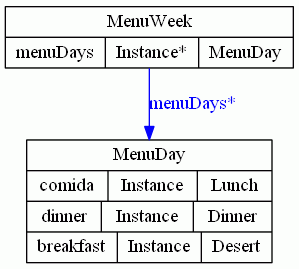
\includegraphics[scale=0.5]{images/classMenu.png}
\caption{Clase Menu}
\label{menu}
\end{figure}

Definimos toda la información de un menú en esta clase. Tenemos la cantidad de días que contiene nuestro plan alimenticio y disitintas instancias de menús diarios los cuales contienen información acerca de sus comidas mediante a sus instancias desayuno, comida y cena. 
\\

Los atributos son: 
\begin{itemize}
\item \textbf{menuDays}: menú diario
\item \textit{comida}: comida de un menú diario
\item \textit{dinner}: cena de un menú diario
\item \textit{breakfast}: desayuno de un menú diario
\end{itemize}

\vspace{0.5cm}

\textbf{class\_Course}
\begin{figure}[H]
\centering
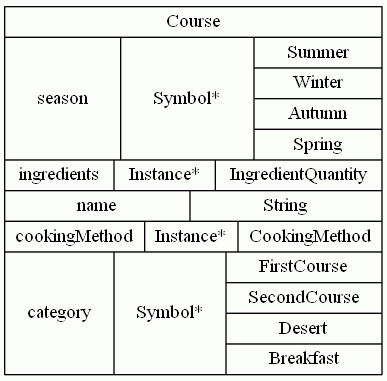
\includegraphics[scale=0.5]{images/classCourse.png}
\caption{Clase Platos}
\label{platos}
\end{figure}

Definimos aquí toda la información que contiene un plato. Tenemos información acerca de qué estación pertenece el plato, los ingredientes que contiene y sus cantidades además de la categoría a la que pertenece que puede ser primer plato, segundo plato, postre o desayuno, 
\\

Los atributos son:
\begin{itemize}
\item \textbf{season}: estación del año; puede ser Otoño, Verano, Invierno o Primavera
\item \textbf{ingredientes}: ingredientes que contiene un plato y su cantidad
\item \textbf{name}: nombre del plato
\item \textbf{category}: categoría del plato; puede ser primer plato, segundo plato, desayuno o postres. 
\end{itemize}


\vspace{0.5cm}

\textbf{class\_Ingredient}
\begin{figure}[H]
\centering
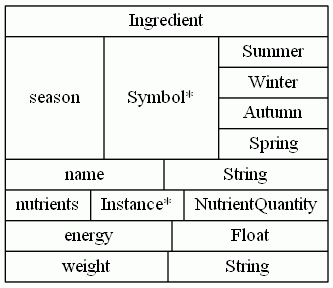
\includegraphics[scale=0.5]{images/classIngredient.png}
\caption{Clase Ingredientes}
\label{ingredientes}
\end{figure}

Definimos aquí toda la información que contiene un ingrediente. Tenemos de manera parecida a los platos, una estación asociada al ingrediente. Por ejemplo: las castañas estarían asociadas al otoño. Además también disponemos de los valores nutricionales que presenta el ingrediente.
\\

Los atributos son: 

\begin{itemize}
\item \textbf{season}: estación del año; puede ser Otoño, Verano, Invierno o Primavera
\item \textbf{name}: nombre del ingrediente
\item \textbf{nutrients}:nutrientes del ingrediente
\end{itemize}


\vspace{0.5cm}

\textbf{class\_IngredientQuantity}
\begin{figure}[H]
\centering
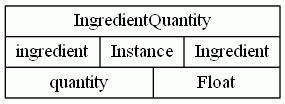
\includegraphics[scale=0.5]{images/classIngredientQuantity.png}
\caption{Clase Enfermedad}
\label{cantidad_ingrediente}
\end{figure}

Para poder expresar la cantidad de ingredientes que contiene un plato hacemos uso de esta clase la cual contiene una referencia a una instancia ingrediente y la cantidad que hay en ese plato del ingrediente.
\\

Los atributos son: 
\begin{itemize}
\item \textbf{ingredient}: ingrediente
\item \textbf{quantity}: cantidad del ingrediente
\end{itemize}


\vspace{0.5cm}

\textbf{class\_Nutrients}
\begin{figure}[H]
\centering
\includegraphics[scale=0.5]{images/classNutrient.png}
\caption{Clase Nutrientes}
\label{nutrientes}
\end{figure}

Definimos en esta clase toda la información que contiene un nutriente... TODO FINISH IT 
\\
TODO continuar amb els atributs
%Los atributos son:
%\begin{itemize}
%\item \textbf{}
%\item \textbf{}
%\end{itemize}


\vspace{0.5cm}

\textbf{class\_NutrientQuantity}
\begin{figure}[H]
\centering
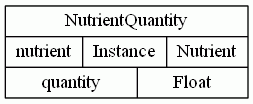
\includegraphics[scale=0.5]{images/classNutrientQuantity.png}
\caption{Clase Cantidad de Nutrientes}
\label{cantidad_nutriente}
\end{figure}

Para poder expresar la cantidad de nutrientes que contiene un ingrediente en concreto hacemos uso de esta clase. Esta dispone de una referencia a una instancia de nutriente además de la cantidad que ese nutriente en ese ingrediente (las unidades han sido normalizadas en gramos). 
\\

Los atributos son: 
\begin{itemize}
\item \textbf{nutrient}: nutriente
\item \textbf{quantity}: cantidad del nutriente
\end{itemize}


\vspace{0.5cm}

\textbf{class\_Disease}
\begin{figure}[H]
\centering
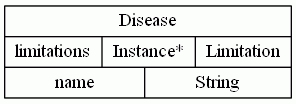
\includegraphics[scale=0.5]{images/classDisease.png}
\caption{Clase Enfermedad}
\label{enfermedad}
\end{figure}

Definimos en esta clase toda la información que contiene una enfermedad. En nuestro caso, una enfermedad presenta una serie de limitaciones alimentícias que pueden estar referidas a un ingrediente o a un tipo de nutriente. 
\\

Los atributos son: 
\begin{itemize}
\item \textbf{limitations}: limitaciones alimentícias que suponen la enfermedad
\item \textbf{name}: nombre de la enfermedad
\end{itemize}


\vspace{0.5cm}

\textbf{class\_Limitation}
\begin{figure}[H]
\centering
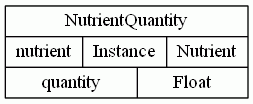
\includegraphics[scale=0.5]{images/classNutrientQuantity.png}
\caption{Clase Limitación}
\label{limitacion}
\end{figure}

Para ser capaces de expresar una limitación o incluso una preferencia alimentícia, hemos hecho uso de esta clase para poder relacionar un nutriente o un ingrediente con una limitación de cantidad AtMost(como máximo) o atLeast(como mínimo).
\\

Los atributos son:
\begin{itemize}
\item \textbf{element}: elemento sobre el que se aplica la limitación, puede ser un nutriente o un ingrediente
\item \textbf{atMost}: valor que representa el tope máximo necesario para cumplir la limitación
\item \textbf{atLeast}: valor que representa el mínimo necesario para cumplir la limitación
\end{itemize}



%explicar detalladamente como se ha construido la ontología

\subsection{Método de resolución}

 explicar problemas que intervienen en la resolución
% Descripción del proceso de resolución y como se organizasn los problemas y subproblemas

\section{Implementación}

\subsection{Creación de la ontología}

Para generar la ontología hemos usado el programa Protégé añadiendo las diferentes características anteriormente mencionadas en los apartados (
%TODO afegir referencia als apartats de desarrollo de ontología)


\section{Juego de Prueba}
%fer-ne més de 6 (lo que consideren un bon número)



%COSES QUE HAURÍEM DE TENIR SEGONS LES RÚBRIQUES 
\subsection{Ejemplos del conocimiento extraído del dominio}
%aquí deberíamos explicar como hemos ido desarrollando prototipos de la implementación para demostrar que hemos usado una metodología incremental 





\end{document}

